\documentclass[../main.tex]{subfiles}

\begin{document}

\chapter{Ghi nhận về thơ đương đại Việt Nam qua một tuyển tập tiếng Anh}

\begin{metadata}

\begin{flushright}27.8.2008\end{flushright}

Paul Hoover

Nguồn: Bài bạt cho cuốn sách Black Dog, Black Night - Contemporary Vietnamese Poetry (Chó đen và đêm - Tuyển tập Thơ Việt Nam đương đại) NXB Milkweed, Hoa Kỳ 2008

\end{metadata}

\begin{multicols}{2}

\begin{figure}
	\centering
	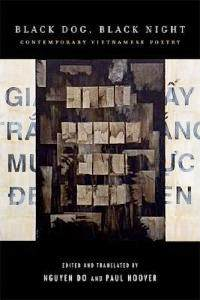
\includegraphics[width=\textwidth]{../img/tho270808.jpg}
	\caption{}
\end{figure}
  Vào tháng 3 và tháng Tư năm 2003, tôi đi du lịch Hà Nội, Huế, Hội An, Sài Gòn trong hai tuần lễ. Nhờ những cố gắng của nhà tiểu thuyết Larry Heinemann và nhà văn Tom Nawrocki ở Chicago, tôi đã gặp được cả Hội Nhà văn đầy quyền lực do Hữu Thỉnh lãnh đạo lẫn nhóm “bên ngoài” (outsiders) do Hoàng Hưng tổ chức. Sự kình địch của hai nhóm lập tức rõ mồn một và ở một mức độ nào đó tìm thấy hình bóng của nó trong đường lối văn chương “inside” (bên trong) và “outside” (bên ngoài) ở Mỹ. Nhưng ở Việt Nam thì hậu quả của sự khác biệt này gay gắt hơn nhiều. Vào thập kỷ 1980, Hoàng Hưng bị giam trong “Hanoi Hilton” và các trại cải tạo chỉ vì bị nghi là sở hữu một bản thảo bị cấm của nhà thơ Hoàng Cầm \footnote{
Thực tế, Hoàng Hưng bị bắt năm 1982 khi cầm trong tay bản thảo tập thơ \textit{Về Kinh Bắc} do Hoàng Cầm chép tặng, với tội danh “lưu truyền văn hoá phẩm phản động”. Đây là một vụ án văn chương kỳ lạ: Từ khi \textit{Về Kinh Bắc} được viết ra (đông xuân 1959-1960) cho đến nay ở Việt Nam chưa từng bao giờ có lệnh cấm sở hữu và lưu truyền bản thảo này, dù là lệnh miệng. Năm 1982, khi có một số nhà văn Việt kiều về xin tập bản thảo này mang đi thì xảy ra vụ án, Hoàng Hưng bị tù 39 tháng, Hoàng Cầm 18 tháng. Sau “Đổi mới”, tập thơ \textit{Về Kinh Bắc} đã được xuất bản và tái bản, những bài quan trọng nhất và “phản động” nhất trong đó (“Cây tam cúc”, “Lá diêu bông”, “Quả vười ổi”) đã góp phần vào tập \textit{Bên kia sông Đuống} - một trong những tập làm nên Giải thưởng Nhà nước về văn học năm 2007 cho Hoàng Cầm. Tuy nhiên, cho tới nay vẫn không ai xem xét lại vụ án này và giải oan cho hai nhà thơ Hoàng Cầm và Hoàng Hưng. “Hanoi Hilton” là tên mà các phi công Mỹ đặt cho trại tạm giam Hoả Lò, Hà Nội, nơi họ bị giam giữ một thời gian trong chiến tranh.} . Được thả trong thời \textit{glasnot \footnote{
Khái niệm “Minh bạch” trong lịch sử đương đại Nga, một yếu tố chính dẫn đến sự sụp đổ của chế độ Xô-viết. Ở đây tác giả muốn nói đến thời “Đổi mới” của Việt Nam.} }, ông trở lại nghề viết báo và  hiện nay là một trong số các nhà thơ và dịch giả hàng đầu của đất nước. Nhưng ông không được hưởng những lợi lộc của một hội viên Hội Nhà văn - những thứ mang đến địa vị, lương bổng và các món lợi khác. 
 
Hội Nhà văn không thể hiếu khách hơn trong cuộc gặp gỡ chúng tôi ở Hà Nội. Sau khi mời trà và giới thiệu tất cả mọi người trong phòng theo truyền thống, Hữu Thỉnh yêu cầu tôi bình luận về tình thế của “Thơ Hậu hiện đại Mỹ”, với tư cách chủ biên tuyển tập của NXB Norton về chủ đề ấy. Các nhà văn có mặt quan tâm nhiều đến những vấn đề trí thức và văn hoá gắn với chủ nghĩa hậu hiện đại. Họ thấy thật trớ trêu khi chủ nghĩa Marx lại có có ảnh hưởng đến lý thuyết văn học của chúng ta \footnote{
Paul Hoover viết cho bạn đọc Mỹ.} . Ba người trong số đó, Nguyễn Duy, Nguyễn Quang Thiều và Hữu Thỉnh, đã được xuất bản bởi Wesleyan University Press và Curbstone Press. Các hội viên đặt nhiều câu hỏi về những thực tế thông thường của việc xuất bản như nhuận bút, bản quyền và giao dịch bản quyền. 
 
Tuyển tập này \footnote{
Paul Hoover là nhà thơ có tên tuổi của Mỹ, chủ biên tuyển tập \textit{Postmodern American Poetry} (Thơ Mỹ Hậu hiện đại) NXB Norton 1994 và cùng với vợ là nhà thơ, nhà văn Maxine Chernoff sáng lập và chủ biên tạp chí \textit{New American Writing} (\textit{Viết Mới}). Hiện là giáo sư khoa Creative Writing (Viết văn) trường San Francisco State University. Đây là bài bạt cho cuốn sách \textit{Black Dog, Black Night - Contemporary Vietnamese Poetry} (Chó đen và đêm - Tuyển tập Thơ Việt Nam đương đại) NXB Milkweed, Hoa Kỳ 2008. Nguyên văn bài viết có tên: “Hanoi Without You: Afterword” (Hà Nội vắng em: Lời bạt) – “Hà Nội vắng em” là tên một bài thơ của Tế Hanh trong tuyển tập, “Chó đen và đêm” là tên một bài thơ của Hoàng Hưng được NXB chọn làm tựa đề chung của tuyển tập. Tập thơ giới thiệu 21 nhà thơ: 17 trong nước (Hữu Loan, Tế Hanh, Văn Cao, Hoàng Cầm, Trần Dần, Đặng Đình Hưng, Nguyễn Khoa Điềm, Xuân Quỳnh, Hoàng Hưng, Trần Vũ Mai, Ý Nhi, Thanh Thảo, Nguyễn Duy, Nguyễn Quang Thiều, Nguyễn Đỗ, Nhật Lệ, Vi Thùy Linh) và 4 là người Mỹ gốc Việt (Đinh Linh, Hoa Nguyen, Truong Tran, Mộng Lan). Tựa đề và các chú thích đều của người dịch.}  bao gồm thơ của các nhà thơ ở cả “bên trong” và “bên ngoài”, nhưng nó cảm thấy đặc biệt có trách nhiệm giới thiệu tác phẩm của các nhà thơ thời kỳ \textit{Nhân văn} và từ đó là những người bị buộc phải viết trong hoàn cảnh bên lề. Đây là tuyển tập thơ đầu tiên xuất bản ở Hoa Kỳ làm việc đó. Thực vậy, cho đến lúc này, thơ Việt Nam xuất bản ở đất nước chúng ta đã đặc biệt là thơ của các hội viên Hội Nhà văn. 
 
Khi Hoàng Hưng đi thăm Hoa Kỳ lần đầu tiên, vào tháng 5 năm 2003, ông giới thiệu tôi với Nguyễn Đỗ - nhà thơ này từ Việt Nam sang ở Sacramento vào cuối thập kỷ 1990. Dự án dịch thơ này là ý tưởng của Đỗ, và ngoại trừ những nhà thơ Mỹ gốc Việt (Đinh Linh, Truong Tran, Mộng Lan và Hoa Nguyen), tất cả những bài thơ đưa vào tuyển là do ông chọn. Nhiệm vụ của tôi là, từ văn bản của ông, tạo nên những bài thơ tiếng Anh tốt nhất có thể. Một số bài đạt được ngay từ vài phác thảo đầu tiên, những bài khác đòi hỏi khá nhiều thay đổi. Ngay từ đầu, thấy rõ là tấn kịch nhân sinh của bài thơ đã nằm sẵn đó hiển nhiên bên dưới cái mặt nạ của sự khác biệt văn hoá. Ngay khi chúng tôi giải thích những thuật ngữ như “young girl rice” \footnote{
Lúa đang thì con gái}  (lúa ngậm sữa ngọt), những ẩn dụ địa phương của các nhà thơ trở nên phổ quát. Cũng như với những bản dịch mới đây về thơ Hölderlin \footnote{
Nhà thơ Đức (1770-1843)}  mà tôi thực hiện với Maxine Chernoff, tôi thấy được sự cần thiết phải đọc vừa cùng với vừa vượt qua văn bản, để tìm kiếm mục tiêu của bài thơ, những sự mỉa mai và đối âm của nó, và đặc biệt là lôgích trí tuệ và cảm xúc của nó. 
 
Sự chọn lựa của chúng tôi nhắm đạt được tính đa dạng và sự tinh khéo của thơ Việt Nam, từ tác phẩm mang tính sáng tạo cao của Đặng Đình Hưng và những người khác, đến cách biểu đạt trữ tình của văn hoá truyền thống của thơ Việt. Sự trung thực và trực tiếp trong diễn đạt mang tính chính trị của thơ Việt Nam rất ấn tượng và có thể dùng làm bài học cho những ai trong chúng ta sống qua cuộc chiến Iraq hiện hành. “Một người lính nói về thế hệ mình” của Thanh Thảo cho ta bức chân dung sống động của đời lính; “Nhìn từ xa Tổ quốc” của Nguyễn Duy thẳng thắn đánh giá tình cảnh đạo đức của đất nước mình trong giai đoạn sau cuộc chiến với Mỹ. Cả hai ông đều ở trong số các nhà thơ nổi tiếng nhất của Việt Nam. Bản dịch những bài thơ của Thanh Thảo của chúng tôi, “12 + 3”, sẽ được xuất bản song ngữ tại Việt Nam với tài trợ của Hội Nhà văn. 
 
Chủ nghĩa hiện đại trong mọi nền văn chương nhấn mạnh sự căng thẳng, đem đến tính tự giác, chủ nghĩa cá nhân, sự khó khăn về trí tuệ và hình thức để kháng cự những truyền thống dân gian: thoải mái, dễ hiểu, và thụ hưởng. Cả hai thứ, truyền thống hiện đại chủ nghĩa và dân gian đều được giới thiệu trong cuốn sách này. Đặng Đình Hưng viết theo lối thơ tự do hậu tượng trưng, giàu liên tưởng, nhưng vẫn duy trì giọng buồn man mác của những bài ca Quan họ. Thơ Hoàng Hưng thấm đượm chủ nghĩa hiện sinh và phong trào Beat \footnote{
Phong trào văn thơ có tinh thần “không tuân phục” ở Mỹ những năm 1950, gồm Jack Kerouac, Allen Ginsberg, William Bourroughs… chủ trương sáng tác theo lối bộc phát.} , nhưng lại dựa trên việc sử dụng giai điệu của các hình thức Quan họ. Sức mạnh và sự thẳng thắn của thơ Nhật Lệ có thể nhắc một số người đọc nghĩ đến những bút pháp tự thú của Sylvia Plath hay Sharon Olds. Sự chân thật và đời sống ngày thường cũng là đặc điểm của thơ Vi Thùy Linh, nhưng khung cảnh và kết cấu thì Việt Nam không nhầm vào đâu được: “My eyes fade like an old praise house” (Mắt tôi phai tàn như một nhà nguyện cũ). Qua cuốn sách này, đó là con chim \textit{khuyên }đang khóc\textit{, }những hạt giống của hoa \textit{lipa }đang bay. Vì thế, thật đáng lưu ý rằng tiếng Việt được dẫn trực tiếp trong cuốn sách này chỉ xuất hiện trong tác phẩm của Truong Tran, nhà thơ này đã sống ở San Francisco từ năm 1975. 
 
Các nhà thơ Mỹ gốc Việt có khác biệt gì quan trọng với những đối tác người Việt của họ không? Cả Đinh Linh và Hoàng Hưng, một Mỹ, một Việt, đều bị hấp dẫn bởi những giọng “tối tăm” tiến gần đến cái thô tục và mộng ảo. Những chất giọng ấy có liên quan đến khuynh hướng, đến ảnh hưởng văn học (Linh hâm mộ Kafka, Hưng bị hấp dẫn bởi Ginsberg), và trải nghiệm sống. Những năm tù đày của Hưng chắc chắn đã làm u tối cuộc đời và thơ ông, nhưng thơ cũng giúp cứu vớt ông. Không có giấy, ông đã luyện trí bằng cách làm thơ trong óc và tự đọc cho mình mình nghe. 
 
Trong một bài tiểu luận, nhà thơ Susan Schultz đã bình về việc sử dụng cái ghê tởm trong thơ Đinh Linh, trong đó có sự “thấu cảm với tư cách ghê tởm”. Sự ghê tởm cũng phối kết với sự kinh ngạc và có thể tìm thấy nguồn gốc trong sự khác biệt văn hoá. Trong bài thơ “Academy of Fine Arts” (Viện Hàn lâm Mỹ thuật), ông diễn đạt niềm tự hào rằng, mặc dù ông cởi truồng, lỗ đít của ông không thòi ra. Điều ấy khiến ông cao cấp hơn loài chó. Trong những bài thơ như thế, Đinh Linh tạo ra những ngụ ngôn xung quanh gương mặt của một kẻ di dân ngỡ ngàng, kinh ngạc vì sự khác biệt về văn hóa và thể chất đối với những người “bản địa” tự mãn xung quanh mình. Trong bài “After Zigzagging” (Sau khi đi vòng vèo), ông viết: “How did I ever learn so many words/ I can’t pronounce?” (Làm thế nào mình học được nhiều từ mà mình không phát âm được thế nhỉ?). Mặt khác, thơ của Hoa Nguyen lại có một giọng điệu cởi mở và đời thường, nhắc nhớ đến những nhà thơ thuộc Trường New York \footnote{
Nhóm nhà thơ tiên phong ở New York trong hai thập kỷ 1950, 1960} . Trong thơ của bà không có sự chia cắt giữa cái tự ngã với thế giới, mà đúng hơn là sự đào sâu một cách sắc sảo cái hiện tại, đặc biệt trong vai trò bí mật nhưng thoải mái của người mẹ. Ngay cái tên của bà, \textit{Hoa, }cũng gợi lên sự mở. Nhưng đặt tên cũng là bắt đầu cho vô số căn tính, đặc biệt đối với một đứa bé lai Âu sinh ra ở Việt Nam: 
\begin{blockquote}
        
\textit{Mã=horse}        
\textit{Mạ=rice seedlings}        
\textit{Mả=grave} 
\textit{Má=mẹ} 

\end{blockquote}
 
Thơ của Truong Tran phối hợp chủ nghĩa hiện đại mang tính thể nghiệm với khao khát bình luận và phản ánh trải nghiệm cá nhân, trong đó có trải nghiệm về căn tính. Trong những bài thơ được chọn ở đây, gương mặt của một người cha vắng mặt, quằn quại, giống như một hồn ma, được tô đậm bằng việc sử dụng hình thức gián đoạn, và trong bài “The Book of Beginnings” (Cuốn sách Khởi đầu), sự vắng mặt các dấu chấm câu đưa đến một giọng điệu bất định mang tính hậu hiện đại. Tác phẩm của Mộng Lan có vẻ ngoài và phạm vi đề tài đã được thấy ở Barbara Guest và Charles Olson, nhưng không chất chứa ý đồ thể nghiệm. Tuy không quá nặng nề, nhưng trong các cấu trúc hình thức mang tính sáng tạo của Truong Tran và Mộng Lan, tính trữ tình và sự tự bi kịch hoá có tham dự vào qui trình. Trong hai nhà thơ, Mộng Lan hướng nhiều hơn về những dáng vẻ triết học như là “night wobbles a drunkard/ at the dialected borders” (đêm lắc lay người say/ ở những biên giới biện chứng). Thơ và chính trị chia sẻ tinh thần của nơi biên giới, chia tách chúng ta giữa quốc gia này với quốc gia khác, cuối cùng là vì lợi ích của cả hai. 
 
Việc giới thiệu các nhà thơ theo trình tự biên niên cho phép bạn đọc chứng kiến sự thay đổi về mỹ học đi đôi với sự phát triển của lịch sử: tầm quan trọng của phong trào Thơ Mới chịu ảnh hưởng của chủ nghĩa lãng mạn Pháp; bước ngoặt về phía mỹ học được chế độ Xô-viết chấp thuận với lối thơ mở rộng và mang tính trình diễn của Maiakovski; lòng dũng cảm của nhóm \textit{Nhân văn} trong thập niên 1950, sự đàn áp về chính trị và sự hồi sinh khuấy động của họ sau năm 1989; những lao khổ của Hoàng Hưng và những người khác trong Chiến tranh Việt-Mỹ, khi những ảnh hưởng ngoại lai, đặc biệt là mô hình kiệt quệ tinh thần hiện sinh chủ nghĩa kiểu Pháp dường như đặc biệt nguy hiểm; và sự ra đời của các nhà thơ nữ trẻ như Nhật Lệ và Vi Thùy Linh trong giai đoạn sau 1989, những người thoải mái biểu đạt mình một cách cá nhân, tính dục và hiện sinh. 
 
Giống như tiếng Hoa, tiếng Việt gồm những từ một âm tiết, cùng với việc sử dụng thanh điệu phức tạp của nó, tạo ra một tiết tấu hoàn toàn khác với những từ đa âm tiết của tiếng Anh. Vì thế, ta không thể tái lập nhịp của một bài thơ tiếng Việt. Ta đành phải dựa vào nhịp của tư duy và giọng điệu. Một số nhà thơ trong sách này sử dụng những thể thơ truyền thống, đó có thể có nghĩa là một số âm tiết nhất định cho mỗi dòng, thường là bốn hay năm. Theo cách đó, dòng thơ năm chữ đầu tiên trong bài “Vọng Tam Hồ” của Hsieh T’iao đọc là:        
\begin{blockquote}
        
Tích thủy chiếu sanh hà (nước tích tụ lại phản chiếu ráng đỏ) \footnote{
Tạ Điều 謝 朓(464~499), người nước Tề thời Nam triều. Bài thơ của ông là \textit{Vọng tam hồ thi }望三湖詩(Chú thích và phiên âm Hán - Việt tên tác giả, tên bài thơ và câu thơ là của GS Nguyễn Huệ Chi)}  

\end{blockquote}
 
Trong tiếng Anh, thể thơ gần gụi nhất với nó mà chúng ta có là “counted verse”, \footnote{
Nghĩa đen: câu thơ được đếm (về số từ/số âm tiết trong câu)}  trong đó số từ chứ không phải số âm tiết nhất định hiện lên ở mỗi dòng thơ. May Swenson, Bob Perelman và Louis Zukofsky cũng như những người khác đã sử dụng thành công thể thơ này. \textit{Counted verse} ưu tiên cho từng từ riêng rẽ. Khi mỗi từ mới đảm nhiệm sức nặng, giá trị và văn cảnh cùng với những từ lân cận, phần còn lại của bài thơ hiệu chỉnh về giọng, sự mở rộng, sự nén, và màu sắc. Không phải mỗi từ được đánh bóng thành trơn tru mang tính trang trí, mà đúng hơn, nó thích hợp cả về quan hệ lẫn sự khác biệt. Được xác quyết hơn, các câu thơ tự chúng sẵn sàng cho sự bày tỏ và thuyết phục. \textit{Counted verse} cho phép một tiết tấu chậm hơn và trực giác hơn của từ, có lẽ vì sức căng giữa sự tùy ý và sự “nhất thiết” của việc chọn lựa từ của nó. 
 
Tôi muốn cảm ơn Nguyễn Đỗ vì tình bạn, tinh thần hợp tác, và vì tấm gương của chính thơ ông. Tôi cũng muốn cảm ơn Hoàng Hưng và các hội viên Hội Nhà văn Hà Nội đã làm cho chuyến đi của tôi thật là vui thích, và cảm ơn Columbia College Chicago đã tài trợ chuyến đi. Tôi biết ơn vì được dự phần làm mới thơ Việt Nam cho người đọc tiếng Anh, họ sẽ thấy một diện rộng các đề tài và phong cách được thực thi ở đó. 
 
 
Bản tiếng Việt © 2008 talawas



\end{multicols}
\end{document}